\documentclass[11pt,a4paper]{article}
\usepackage[T1]{fontenc}
\usepackage[margin=2cm]{geometry}
\usepackage{graphicx}
\graphicspath{{figures/}{modelling_optimisation/paper/figures/}}
\usepackage[hidelinks]{hyperref}
\setlength{\parindent}{0pt}
\setlength{\parskip}{0.7em}
\title{General maps of the modelling framework}
\author{}
\date{}
\begin{document}
\maketitle
\vspace{-2em}
\textbf{1. Overall workflow --- suggested main-paper figure.}

This map gives the general idea of the code: physical model, radiative transfer,
observable comparison and parameter search. It is independent of a particular
disc prescription, parameter range or experiment. Use it as a two-column figure.

\begin{figure}[htbp]
\centering
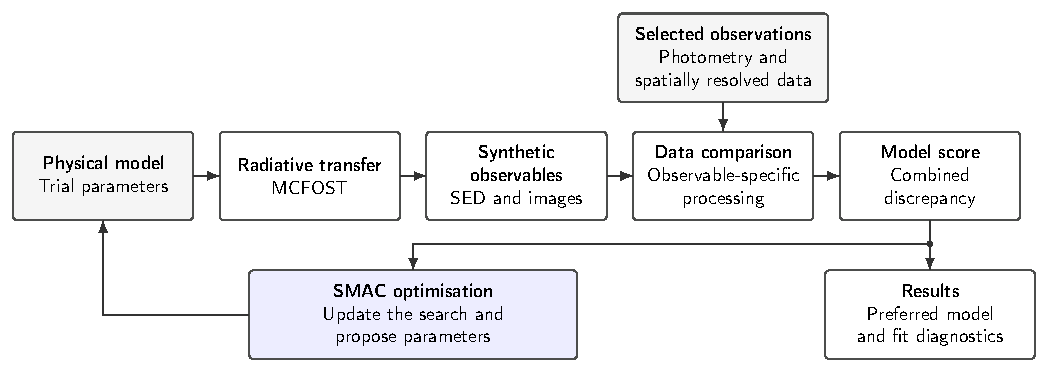
\includegraphics[width=\linewidth]{model_map_workflow.pdf}
\caption{Overview of the modelling and optimisation framework. A trial physical
model is evaluated with MCFOST and compared with the selected observations
after observable-specific processing. The combined discrepancy guides the
SMAC parameter search. The final outputs include the preferred model and
diagnostics for the individual observables.}
\end{figure}

\textbf{Inserting the figures.}
The files in \texttt{figures/} are cropped vector PDFs and can be included with
\verb|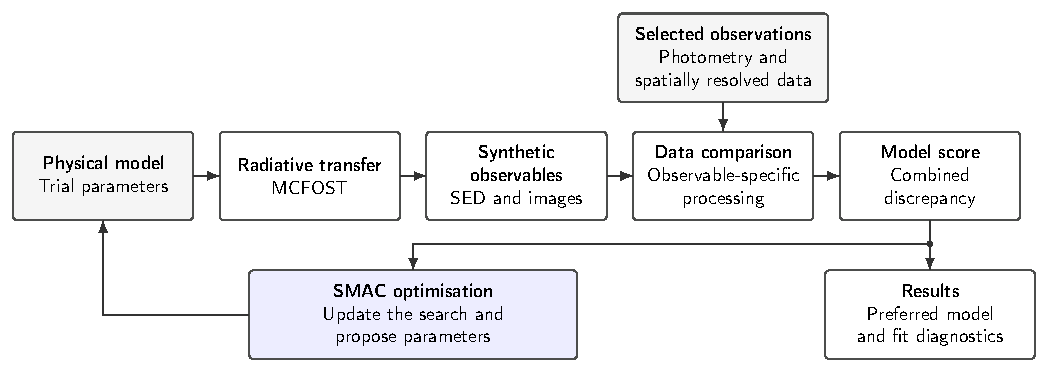
\includegraphics[width=\linewidth]{model_map_workflow.pdf}|.
Each PDF has a matching, independently compilable \texttt{.tex} source.
The figure PDFs contain only the diagrams, so their captions can follow
the journal's style.

\clearpage
\textbf{2. Physical-model overview.}

This map is suitable for the physical-model section. It shows the main input
groups and the products of the radiative-transfer calculation without assigning
numerical values or distinguishing fixed from fitted parameters.

\begin{figure}[htbp]
\centering
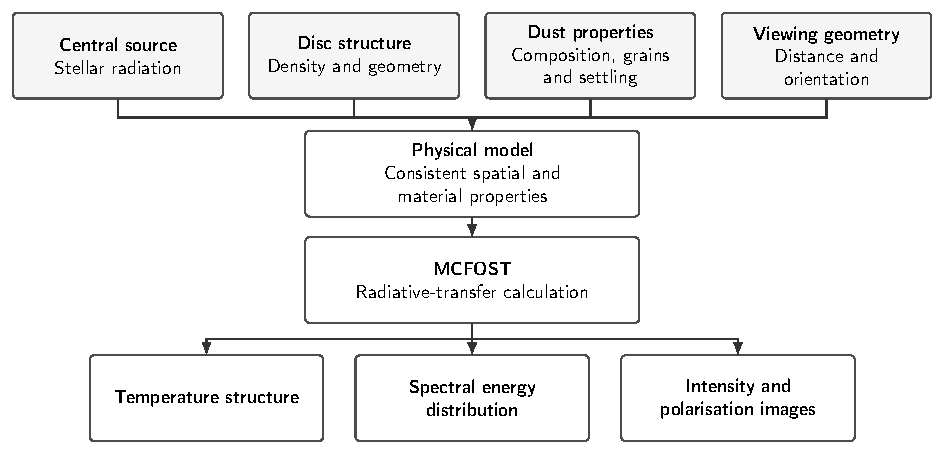
\includegraphics[width=\linewidth]{model_map_physical.pdf}
\caption{Physical inputs and radiative-transfer products. The central source,
disc structure, dust properties and viewing geometry define a model evaluated
with MCFOST. The calculation provides the temperature structure, spectral energy
distribution, and intensity and polarisation images.}
\end{figure}

\clearpage
\textbf{3. Observable-comparison overview.}

This map is suitable for the comparison-methods section. The four branches are
alternative or complementary constraints. Only the selected branches contribute
to a given experiment; the diagram does not imply a staged optimisation.

\begin{figure}[htbp]
\centering
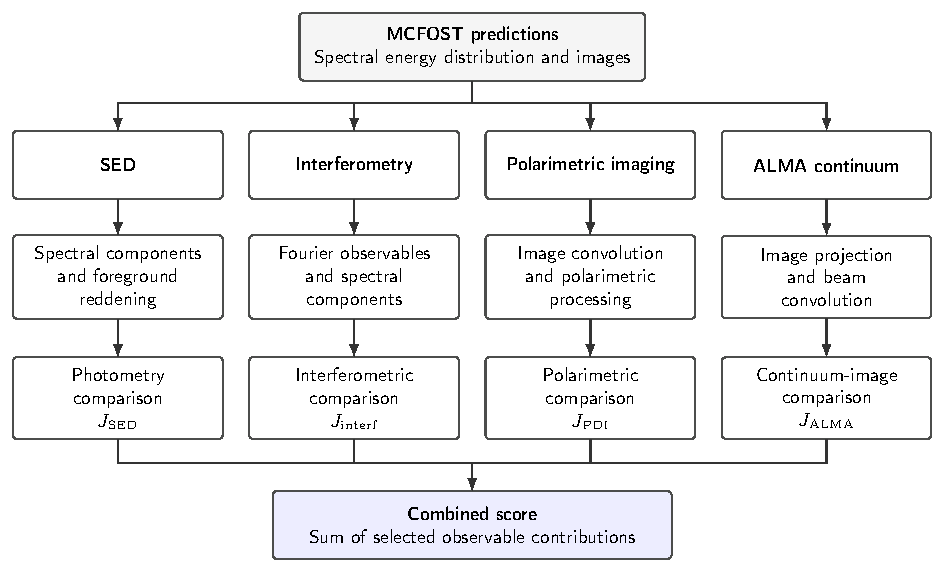
\includegraphics[width=\linewidth]{model_map_observables.pdf}
\caption{Observable-specific comparison of model predictions with the data.
Synthetic spectra and images undergo the processing appropriate to each
observable before comparison with the corresponding observations.
The selected discrepancy terms are summed to form the optimisation score.
The interferometric and polarimetric terms include their instrument or band
contributions.}
\end{figure}

The score is a composite discrepancy measure. The diagram does not imply
identical statistical definitions or equal numerical weights for its components.
\end{document}
